% Options for packages loaded elsewhere
\PassOptionsToPackage{unicode}{hyperref}
\PassOptionsToPackage{hyphens}{url}
%
\documentclass[
]{article}
\usepackage{amsmath,amssymb}
\usepackage{lmodern}
\usepackage{iftex}
\ifPDFTeX
  \usepackage[T1]{fontenc}
  \usepackage[utf8]{inputenc}
  \usepackage{textcomp} % provide euro and other symbols
\else % if luatex or xetex
  \usepackage{unicode-math}
  \defaultfontfeatures{Scale=MatchLowercase}
  \defaultfontfeatures[\rmfamily]{Ligatures=TeX,Scale=1}
\fi
% Use upquote if available, for straight quotes in verbatim environments
\IfFileExists{upquote.sty}{\usepackage{upquote}}{}
\IfFileExists{microtype.sty}{% use microtype if available
  \usepackage[]{microtype}
  \UseMicrotypeSet[protrusion]{basicmath} % disable protrusion for tt fonts
}{}
\makeatletter
\@ifundefined{KOMAClassName}{% if non-KOMA class
  \IfFileExists{parskip.sty}{%
    \usepackage{parskip}
  }{% else
    \setlength{\parindent}{0pt}
    \setlength{\parskip}{6pt plus 2pt minus 1pt}}
}{% if KOMA class
  \KOMAoptions{parskip=half}}
\makeatother
\usepackage{xcolor}
\usepackage[margin=1in]{geometry}
\usepackage{color}
\usepackage{fancyvrb}
\newcommand{\VerbBar}{|}
\newcommand{\VERB}{\Verb[commandchars=\\\{\}]}
\DefineVerbatimEnvironment{Highlighting}{Verbatim}{commandchars=\\\{\}}
% Add ',fontsize=\small' for more characters per line
\usepackage{framed}
\definecolor{shadecolor}{RGB}{248,248,248}
\newenvironment{Shaded}{\begin{snugshade}}{\end{snugshade}}
\newcommand{\AlertTok}[1]{\textcolor[rgb]{0.94,0.16,0.16}{#1}}
\newcommand{\AnnotationTok}[1]{\textcolor[rgb]{0.56,0.35,0.01}{\textbf{\textit{#1}}}}
\newcommand{\AttributeTok}[1]{\textcolor[rgb]{0.77,0.63,0.00}{#1}}
\newcommand{\BaseNTok}[1]{\textcolor[rgb]{0.00,0.00,0.81}{#1}}
\newcommand{\BuiltInTok}[1]{#1}
\newcommand{\CharTok}[1]{\textcolor[rgb]{0.31,0.60,0.02}{#1}}
\newcommand{\CommentTok}[1]{\textcolor[rgb]{0.56,0.35,0.01}{\textit{#1}}}
\newcommand{\CommentVarTok}[1]{\textcolor[rgb]{0.56,0.35,0.01}{\textbf{\textit{#1}}}}
\newcommand{\ConstantTok}[1]{\textcolor[rgb]{0.00,0.00,0.00}{#1}}
\newcommand{\ControlFlowTok}[1]{\textcolor[rgb]{0.13,0.29,0.53}{\textbf{#1}}}
\newcommand{\DataTypeTok}[1]{\textcolor[rgb]{0.13,0.29,0.53}{#1}}
\newcommand{\DecValTok}[1]{\textcolor[rgb]{0.00,0.00,0.81}{#1}}
\newcommand{\DocumentationTok}[1]{\textcolor[rgb]{0.56,0.35,0.01}{\textbf{\textit{#1}}}}
\newcommand{\ErrorTok}[1]{\textcolor[rgb]{0.64,0.00,0.00}{\textbf{#1}}}
\newcommand{\ExtensionTok}[1]{#1}
\newcommand{\FloatTok}[1]{\textcolor[rgb]{0.00,0.00,0.81}{#1}}
\newcommand{\FunctionTok}[1]{\textcolor[rgb]{0.00,0.00,0.00}{#1}}
\newcommand{\ImportTok}[1]{#1}
\newcommand{\InformationTok}[1]{\textcolor[rgb]{0.56,0.35,0.01}{\textbf{\textit{#1}}}}
\newcommand{\KeywordTok}[1]{\textcolor[rgb]{0.13,0.29,0.53}{\textbf{#1}}}
\newcommand{\NormalTok}[1]{#1}
\newcommand{\OperatorTok}[1]{\textcolor[rgb]{0.81,0.36,0.00}{\textbf{#1}}}
\newcommand{\OtherTok}[1]{\textcolor[rgb]{0.56,0.35,0.01}{#1}}
\newcommand{\PreprocessorTok}[1]{\textcolor[rgb]{0.56,0.35,0.01}{\textit{#1}}}
\newcommand{\RegionMarkerTok}[1]{#1}
\newcommand{\SpecialCharTok}[1]{\textcolor[rgb]{0.00,0.00,0.00}{#1}}
\newcommand{\SpecialStringTok}[1]{\textcolor[rgb]{0.31,0.60,0.02}{#1}}
\newcommand{\StringTok}[1]{\textcolor[rgb]{0.31,0.60,0.02}{#1}}
\newcommand{\VariableTok}[1]{\textcolor[rgb]{0.00,0.00,0.00}{#1}}
\newcommand{\VerbatimStringTok}[1]{\textcolor[rgb]{0.31,0.60,0.02}{#1}}
\newcommand{\WarningTok}[1]{\textcolor[rgb]{0.56,0.35,0.01}{\textbf{\textit{#1}}}}
\usepackage{longtable,booktabs,array}
\usepackage{calc} % for calculating minipage widths
% Correct order of tables after \paragraph or \subparagraph
\usepackage{etoolbox}
\makeatletter
\patchcmd\longtable{\par}{\if@noskipsec\mbox{}\fi\par}{}{}
\makeatother
% Allow footnotes in longtable head/foot
\IfFileExists{footnotehyper.sty}{\usepackage{footnotehyper}}{\usepackage{footnote}}
\makesavenoteenv{longtable}
\usepackage{graphicx}
\makeatletter
\def\maxwidth{\ifdim\Gin@nat@width>\linewidth\linewidth\else\Gin@nat@width\fi}
\def\maxheight{\ifdim\Gin@nat@height>\textheight\textheight\else\Gin@nat@height\fi}
\makeatother
% Scale images if necessary, so that they will not overflow the page
% margins by default, and it is still possible to overwrite the defaults
% using explicit options in \includegraphics[width, height, ...]{}
\setkeys{Gin}{width=\maxwidth,height=\maxheight,keepaspectratio}
% Set default figure placement to htbp
\makeatletter
\def\fps@figure{htbp}
\makeatother
\setlength{\emergencystretch}{3em} % prevent overfull lines
\providecommand{\tightlist}{%
  \setlength{\itemsep}{0pt}\setlength{\parskip}{0pt}}
\setcounter{secnumdepth}{-\maxdimen} % remove section numbering
\ifLuaTeX
  \usepackage{selnolig}  % disable illegal ligatures
\fi
\IfFileExists{bookmark.sty}{\usepackage{bookmark}}{\usepackage{hyperref}}
\IfFileExists{xurl.sty}{\usepackage{xurl}}{} % add URL line breaks if available
\urlstyle{same} % disable monospaced font for URLs
\hypersetup{
  pdftitle={Predicting the revenue of the movies based on budget},
  hidelinks,
  pdfcreator={LaTeX via pandoc}}

\title{Predicting the revenue of the movies based on budget}
\author{}
\date{\vspace{-2.5em}}

\begin{document}
\maketitle

\begin{Shaded}
\begin{Highlighting}[]
\FunctionTok{library}\NormalTok{(here)}
\end{Highlighting}
\end{Shaded}

\begin{verbatim}
## here() starts at /home/rstudio
\end{verbatim}

\begin{Shaded}
\begin{Highlighting}[]
\FunctionTok{library}\NormalTok{(tidyverse)}
\end{Highlighting}
\end{Shaded}

\begin{verbatim}
## -- Attaching core tidyverse packages ------------------------ tidyverse 2.0.0 --
## v dplyr     1.1.0     v readr     2.1.4
## v forcats   1.0.0     v stringr   1.5.0
## v ggplot2   3.4.1     v tibble    3.2.0
## v lubridate 1.9.2     v tidyr     1.3.0
## v purrr     1.0.1
\end{verbatim}

\begin{verbatim}
## -- Conflicts ------------------------------------------ tidyverse_conflicts() --
## x dplyr::filter() masks stats::filter()
## x dplyr::lag()    masks stats::lag()
## i Use the ]8;;http://conflicted.r-lib.org/conflicted package]8;; to force all conflicts to become errors
\end{verbatim}

\begin{Shaded}
\begin{Highlighting}[]
\FunctionTok{library}\NormalTok{(repr)}
\FunctionTok{library}\NormalTok{(tidymodels)}
\end{Highlighting}
\end{Shaded}

\begin{verbatim}
## -- Attaching packages -------------------------------------- tidymodels 1.0.0 --
## v broom        1.0.4     v rsample      1.1.1
## v dials        1.1.0     v tune         1.0.1
## v infer        1.0.4     v workflows    1.1.3
## v modeldata    1.1.0     v workflowsets 1.0.0
## v parsnip      1.0.4     v yardstick    1.1.0
## v recipes      1.0.5     
## -- Conflicts ----------------------------------------- tidymodels_conflicts() --
## x scales::discard() masks purrr::discard()
## x dplyr::filter()   masks stats::filter()
## x recipes::fixed()  masks stringr::fixed()
## x dplyr::lag()      masks stats::lag()
## x yardstick::spec() masks readr::spec()
## x recipes::step()   masks stats::step()
## * Search for functions across packages at https://www.tidymodels.org/find/
\end{verbatim}

\begin{Shaded}
\begin{Highlighting}[]
\FunctionTok{library}\NormalTok{(GGally)}
\end{Highlighting}
\end{Shaded}

\begin{verbatim}
## Registered S3 method overwritten by 'GGally':
##   method from   
##   +.gg   ggplot2
\end{verbatim}

\begin{Shaded}
\begin{Highlighting}[]
\FunctionTok{library}\NormalTok{(infer)}
\FunctionTok{library}\NormalTok{(cowplot)}
\end{Highlighting}
\end{Shaded}

\begin{verbatim}
## 
## Attaching package: 'cowplot'
## 
## The following object is masked from 'package:lubridate':
## 
##     stamp
\end{verbatim}

By - Rehan Mondal and Abheet Kansal Adapted from DSCI 100 Project by -
Ming Zhang, Rehan Mondal, Caroline Lu and Jingwen Leng

\hypertarget{summary}{%
\subsection{Summary}\label{summary}}

The project deals with predicting whether movies with high budget have
high revenue. The project tries to correlate the impact the amount of
money spent in making a movie has on the revenue it generates.

\hypertarget{introduction}{%
\subsection{Introduction}\label{introduction}}

The entertainment industry has always been a profitable field,
especially movies. However, with great profit comes great investment.
Most modern-day movies require a budget of around 100 million
dollars(1). It is crucial for investors/directors to have a general idea
of how much profit they can make based on their investment. Thus, this
project centers around studying the profitability of a movie before it
is released, predicting revenues based on budget using Knn regression
(since most movies fall under a general range of budget and there are
rarely extreme outliers)

The question we will try to answer with our project is what is the
revenue of a movie based on budget. The data set, which consists of 5000
movies from TMDB, will be separated into training and testing sets.
Using budget as the predictor, the prediction of test set revenue will
be made.

In the data set ``TMDB 5000 Movie Dataset'' (from
``\url{https://www.kaggle.com/datasets/tmdb/tmdb-movie-metadata}''),
revenues, budget, popularity are recorded for the 5000 movies listed in
an excel format. Other columns are listed/included in the data set as
well, however because they are written in json or not a significant
predictor to the revenue, those columns will be filtered out. Revenues
is defined as the total box income of the movie; budget is defined as
the funding used for the production; Popularity numbers are built
according to the TMDB model which consists of number of votes for the
day, number of views for the day, number of users who marked it as a
``favourite'' for the day, Number of users who added it to their
``watchlist'' for the day, release date, number of total votes, and
previous days score. We will discuss and analyze the correlation of each
variable with revenue below.

\hypertarget{methods-results}{%
\subsection{Methods \& Results:}\label{methods-results}}

We used functions from the tidyverse library to manipulate data frames
and tibbles. repr is used to resize plots contained in this notebook,
such as an ``Accuracy vs K'' graph. tidymodels is a package used for
statistical and modeling analysis. GGally extends ggplot2 by adding
several functions to reduce the complexity of combining geoms with
transformed data. cowplot is used to generate the function plot-grid to
easily compare plots.

\begin{Shaded}
\begin{Highlighting}[]
\NormalTok{data }\OtherTok{\textless{}{-}} \FunctionTok{read.csv}\NormalTok{(}\StringTok{"data/dataset.csv"}\NormalTok{)}
\end{Highlighting}
\end{Shaded}

\begin{Shaded}
\begin{Highlighting}[]
\NormalTok{clean\_data }\OtherTok{\textless{}{-}} \FunctionTok{read.csv}\NormalTok{(}\StringTok{"data/clean\_dataset.csv"}\NormalTok{)}
\NormalTok{clean\_data }\OtherTok{\textless{}{-}} \FunctionTok{head}\NormalTok{(clean\_data)}
\NormalTok{knitr}\SpecialCharTok{::}\FunctionTok{kable}\NormalTok{(clean\_data, }\AttributeTok{caption =} \StringTok{"TMDB rating"}\NormalTok{)}
\end{Highlighting}
\end{Shaded}

\begin{longtable}[]{@{}rrrrrr@{}}
\caption{TMDB rating}\tabularnewline
\toprule()
X & budget & revenue & vote\_average & runtime & popularity \\
\midrule()
\endfirsthead
\toprule()
X & budget & revenue & vote\_average & runtime & popularity \\
\midrule()
\endhead
1 & 2.37e+08 & 2787965087 & 7.2 & 162 & 150.43758 \\
2 & 3.00e+08 & 961000000 & 6.9 & 169 & 139.08262 \\
3 & 2.45e+08 & 880674609 & 6.3 & 148 & 107.37679 \\
4 & 2.50e+08 & 1084939099 & 7.6 & 165 & 112.31295 \\
5 & 2.60e+08 & 284139100 & 6.1 & 132 & 43.92699 \\
6 & 2.58e+08 & 890871626 & 5.9 & 139 & 115.69981 \\
\bottomrule()
\end{longtable}

As of now, we have a single giant data frame consisting of all the data
of TMDB movie. If we pass all of the revenue data into our model, we
would not have any data to use as a measure of how accurate the model
is. If we use the data that we have used to train the model before, the
model will recognize that data because it has ``seen'' it before and
will most likely produce a faulty accuracy that is higher than reality.

Therefore, to allow a fair process of measuring the model's accuracy, we
must calculate its accuracy based on how accurate it is at predicting
revenues that it hasn't ``seen'' before. To do this, we split the data
into training and testing datasets and only use the training dataset to
create our regression model. By doing so, we will have a set of data
that the machine learning hasn't seen before.

To do this, we will use the golden ratio which is a 75-25\% ratio of
training and testing datasets respectively. The strata statement can
shuffle and ensure the data is not split unrepresentatively.

To make sure that this process is replicable, we use set.seed().

\begin{Shaded}
\begin{Highlighting}[]
\CommentTok{\# Graph for train data}
\NormalTok{knitr}\SpecialCharTok{::}\FunctionTok{include\_graphics}\NormalTok{(}\StringTok{"data/initial\_scatter\_plot.jpeg"}\NormalTok{)}
\end{Highlighting}
\end{Shaded}

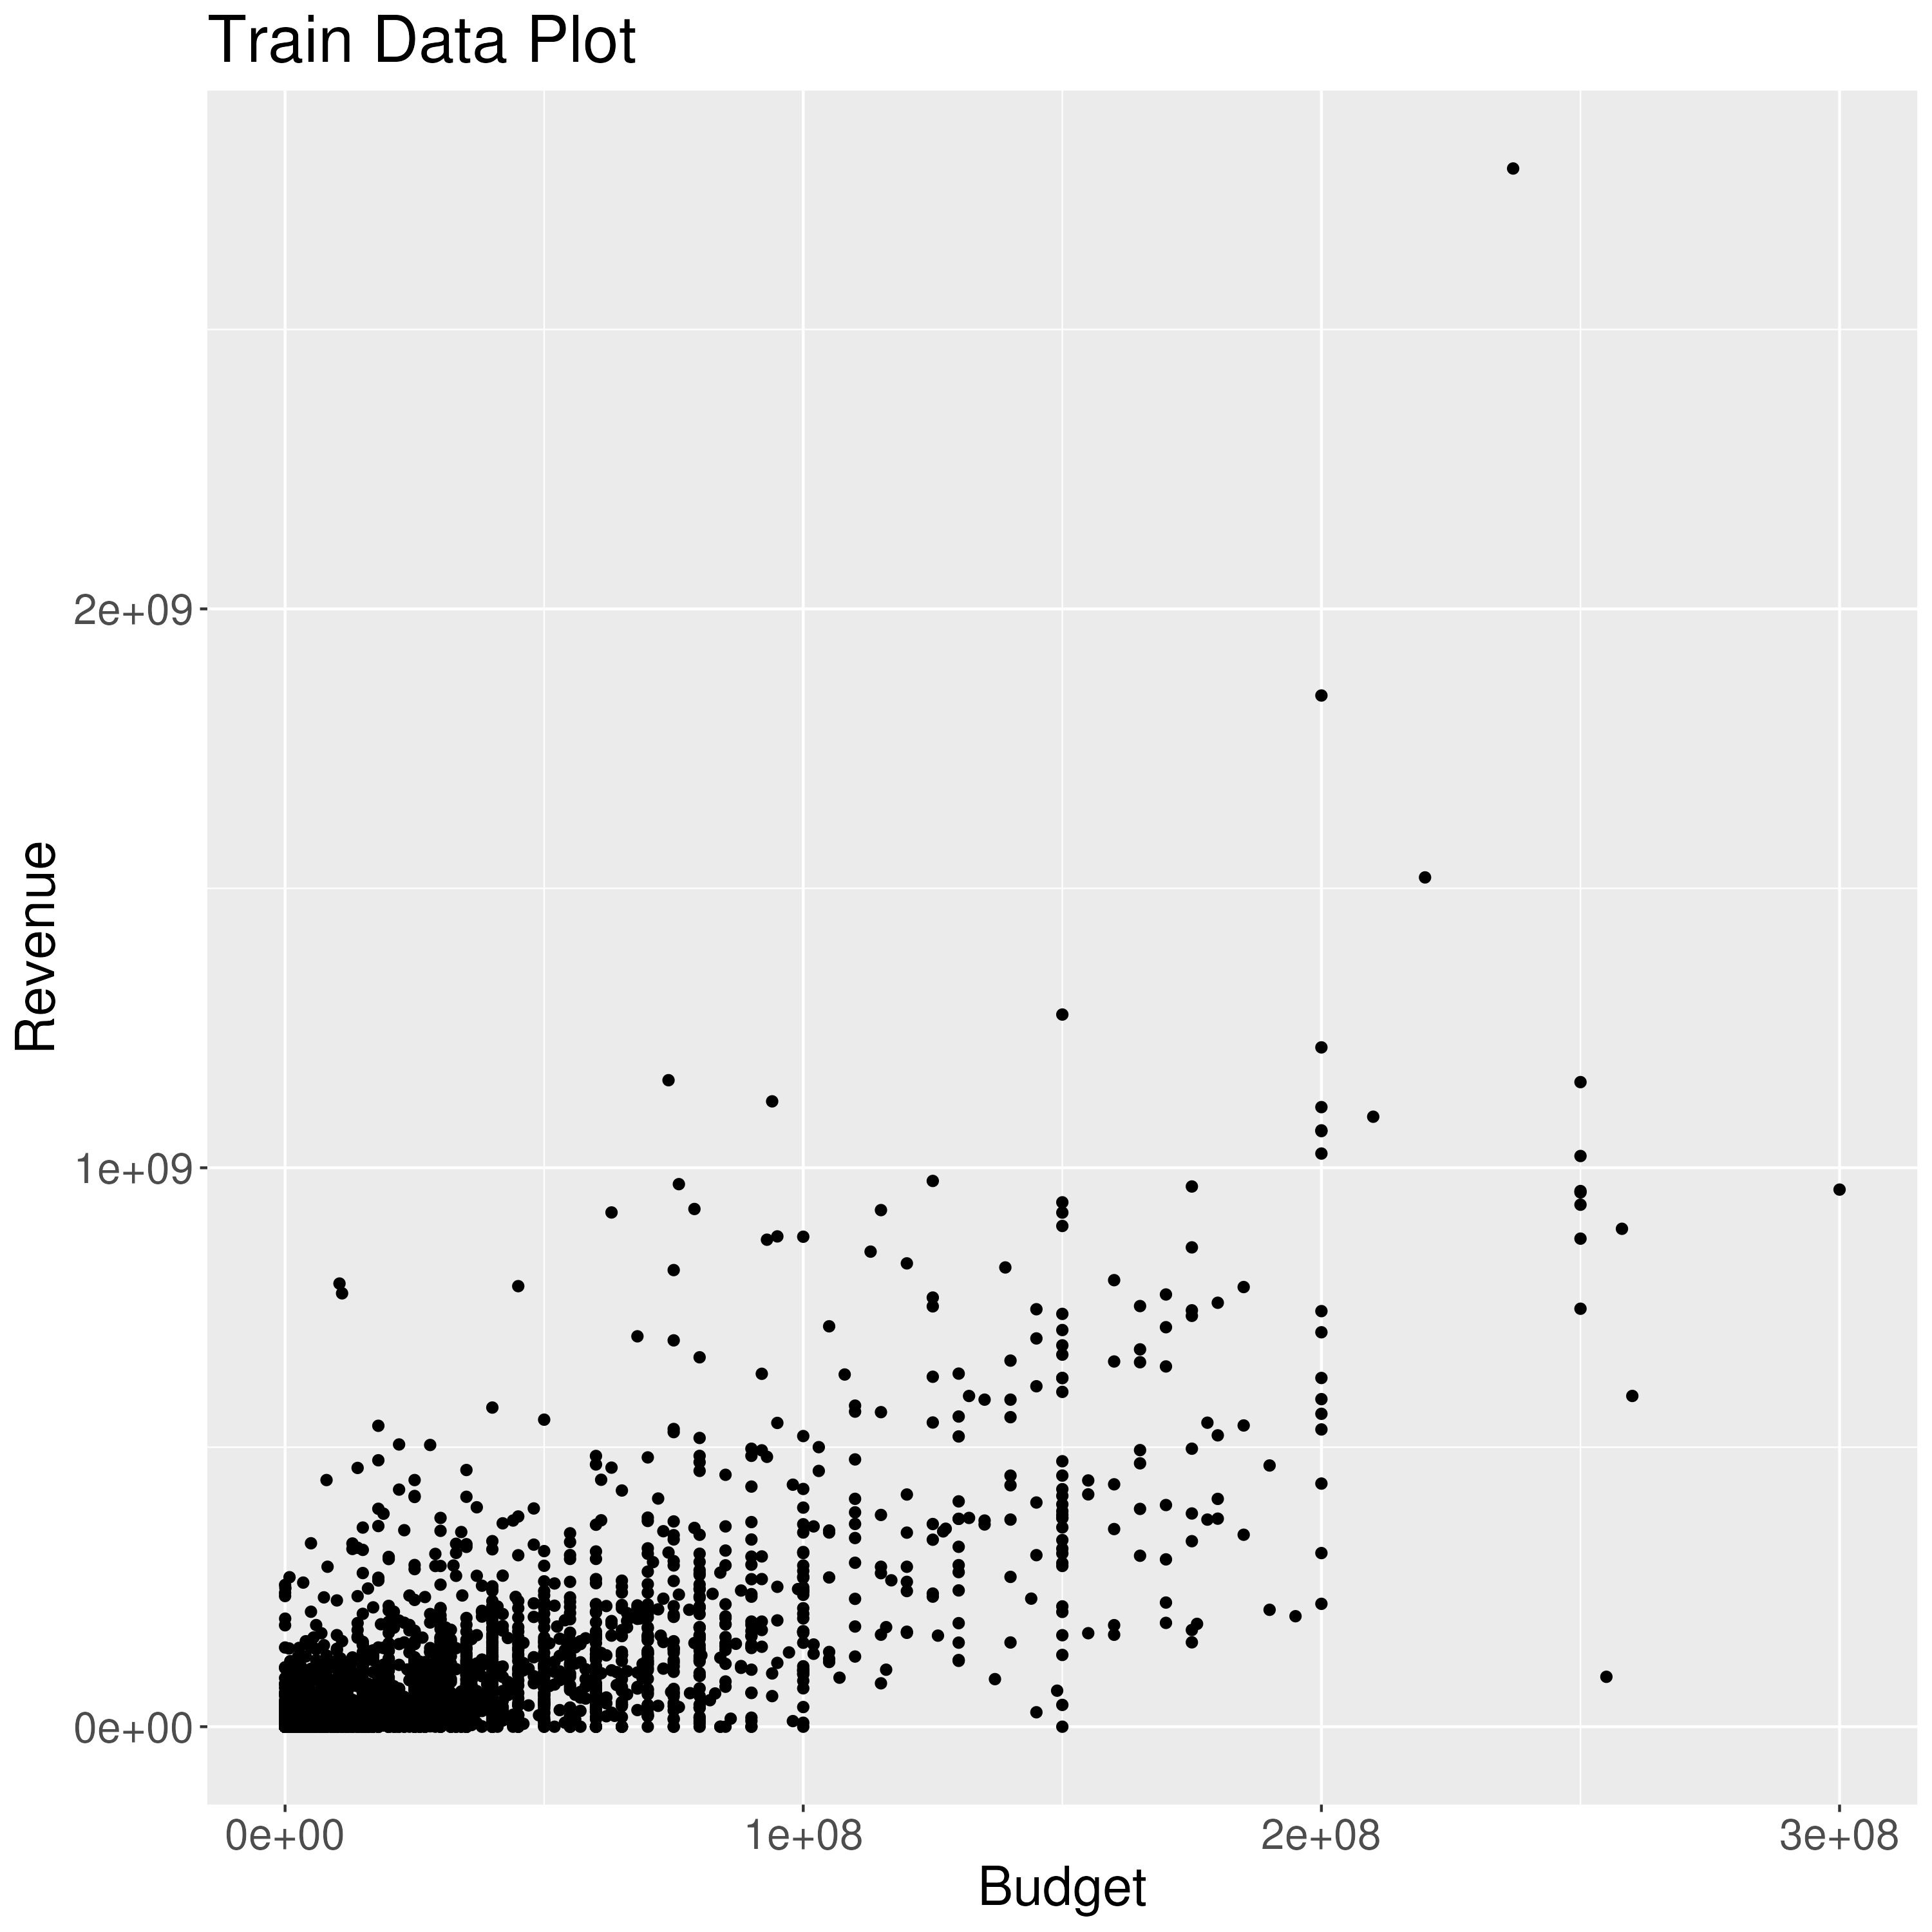
\includegraphics{data/initial_scatter_plot.jpeg}

Below we use ggpairs to analyze the correlation between revenues and the
predictors ``vote\_average'', ``budget'', ``runtime'', and
``popularity''.

As we can see, the correlation between budget and revenue is the
strongest, and it is also our subject of interest since we are trying to
predict revenues based off budget which can directly influence the
profit of the investors. All the other predictos have little to no
correlation with revenues. Other predictos such as popularity are only
relevant or in-existence after the production of the movie which are
also not reliable predictors to understand revenue before the
investment. For example, Popularity numbers are built according to the
TMDB model which consists of number of votes for the day, number of
views for the day, number of users who marked it as a ``favourite'' for
the day, Number of users who added it to their ``watchlist'' for the
day, release date, number of total votes, and previous days score (which
are only recorded after the movie is produced).

\begin{Shaded}
\begin{Highlighting}[]
\NormalTok{ knitr}\SpecialCharTok{::}\FunctionTok{include\_graphics}\NormalTok{(}\StringTok{"data/cp.jpeg"}\NormalTok{)}
\end{Highlighting}
\end{Shaded}

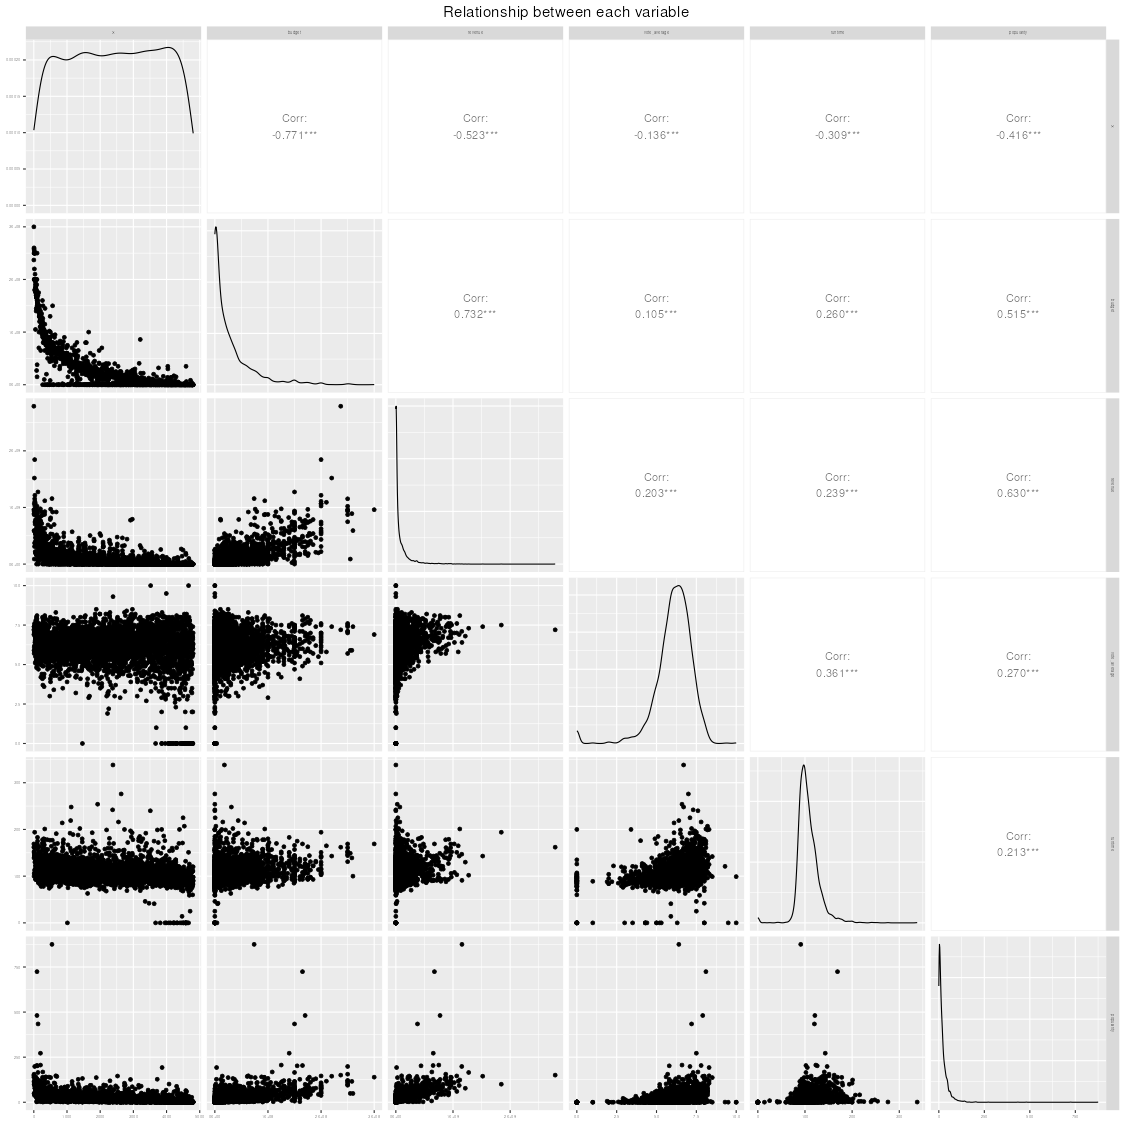
\includegraphics{data/cp.jpeg}

\hypertarget{knn-nearest-neighbor-regression-model-training}{%
\subsubsection{Knn-nearest neighbor regression model
training}\label{knn-nearest-neighbor-regression-model-training}}

First, we created a recipe using the recipe functions with the variables
of interest \texttt{budget} using the training dataset and assign your
answer to an object named revenue\_recipe. We also thought of scaling
\texttt{step\_scale} and centering \texttt{step\_center} steps for all
of the predictors so that they each have a mean of 0 and standard
deviation of 1, but it was not necessary because we only have one
predictor, and standardization can cause a loss of interpretation.

If we split our overall training data once, our best parameter choice
will depend strongly on our luck (since whatever data that lands in the
validation set is random). By using multiple different train /
validation splits, a better accuracy/representation of the data can be
estimated, which will lead to a better choice of the number of
neighbours \(K\) for the overall set of training data.

In cross-validation, we split our overall training data into \(x\)
evenly-sized chunks, and then iteratively use 1 chunk as the validation
set and combine the remaining \(x-1\) chunks as the training set.

We decided to split our overall training data up in multiple different
ways using \texttt{vfold\_cv}, train and evaluate a regression model for
each split, and then choose the parameter based on all of the different
results. The v value is set as 5 which is the number of folds, and we
set revenue as the strata arguement.

We created \textbf{revenue\_spec} using the \texttt{nearest\_neighbor}
function.

In order to improve our regression model, we need to change the
parameter: number of neighbours, \(K\). Since cross-validation helps us
evaluate the accuracy of our model, we can use cross-validation to pick
the value of \(K\) that gives us the best accuracy.

Using \texttt{tune()} in \texttt{tidymodels} package, each parameter in
the model can be altered/attempted rather than given a specific value.

Using \texttt{workflow}, we can chain together multiple data analysis
steps without a lot of otherwise necessary code for intermediate steps.
We use the \textbf{revenue\_recipe} and \textbf{revenue\_spec} we have
created previously in the workflow.

We can use \texttt{tibble} to create a set of values we will be using
for the grid arguement (the range of parameter we will be testing).
Here, we indicated the \(K\) value to range from 1 to 500, and step by
2.

We can then use the tune\_grid function to fit the model for each value
in a range of parameter values. For the resamples argument, we input the
cross-validation revenue\_vfold we created earlier. The grid argument
specifies that the tuning should try \(X\) amount of values of the
number of neighbors \(K\) when tuning, we input the gridvals object we
created earlier to indicate the range of parameters we would like to
try.

We then used filter to only list out rmse (which represent \(RMSE\):
root mean square prediction error) to use to evaluate for the best k
value.

\begin{Shaded}
\begin{Highlighting}[]
\CommentTok{\# Plot K Values}
\NormalTok{knitr}\SpecialCharTok{::}\FunctionTok{include\_graphics}\NormalTok{(}\StringTok{"data/K{-}value\_plot.jpeg"}\NormalTok{)}
\end{Highlighting}
\end{Shaded}

\includegraphics{data/K-value_plot.jpeg}

Here we can see neighbor \(K = 85\) gives us the minimum \(RMSE\).

\begin{Shaded}
\begin{Highlighting}[]
\CommentTok{\# Exact K value}
\NormalTok{minK }\OtherTok{\textless{}{-}} \FunctionTok{read.csv}\NormalTok{(}\StringTok{"data/minK.csv"}\NormalTok{)}
\NormalTok{knitr}\SpecialCharTok{::}\FunctionTok{kable}\NormalTok{(minK, }\AttributeTok{caption =} \StringTok{"Minimum Value of K"}\NormalTok{)     }
\end{Highlighting}
\end{Shaded}

\begin{longtable}[]{@{}
  >{\raggedleft\arraybackslash}p{(\columnwidth - 14\tabcolsep) * \real{0.0395}}
  >{\raggedleft\arraybackslash}p{(\columnwidth - 14\tabcolsep) * \real{0.1316}}
  >{\raggedright\arraybackslash}p{(\columnwidth - 14\tabcolsep) * \real{0.1053}}
  >{\raggedright\arraybackslash}p{(\columnwidth - 14\tabcolsep) * \real{0.1447}}
  >{\raggedleft\arraybackslash}p{(\columnwidth - 14\tabcolsep) * \real{0.1316}}
  >{\raggedleft\arraybackslash}p{(\columnwidth - 14\tabcolsep) * \real{0.0395}}
  >{\raggedleft\arraybackslash}p{(\columnwidth - 14\tabcolsep) * \real{0.1053}}
  >{\raggedright\arraybackslash}p{(\columnwidth - 14\tabcolsep) * \real{0.3026}}@{}}
\caption{Minimum Value of K}\tabularnewline
\toprule()
\begin{minipage}[b]{\linewidth}\raggedleft
X
\end{minipage} & \begin{minipage}[b]{\linewidth}\raggedleft
neighbors
\end{minipage} & \begin{minipage}[b]{\linewidth}\raggedright
.metric
\end{minipage} & \begin{minipage}[b]{\linewidth}\raggedright
.estimator
\end{minipage} & \begin{minipage}[b]{\linewidth}\raggedleft
mean
\end{minipage} & \begin{minipage}[b]{\linewidth}\raggedleft
n
\end{minipage} & \begin{minipage}[b]{\linewidth}\raggedleft
std\_err
\end{minipage} & \begin{minipage}[b]{\linewidth}\raggedright
.config
\end{minipage} \\
\midrule()
\endfirsthead
\toprule()
\begin{minipage}[b]{\linewidth}\raggedleft
X
\end{minipage} & \begin{minipage}[b]{\linewidth}\raggedleft
neighbors
\end{minipage} & \begin{minipage}[b]{\linewidth}\raggedright
.metric
\end{minipage} & \begin{minipage}[b]{\linewidth}\raggedright
.estimator
\end{minipage} & \begin{minipage}[b]{\linewidth}\raggedleft
mean
\end{minipage} & \begin{minipage}[b]{\linewidth}\raggedleft
n
\end{minipage} & \begin{minipage}[b]{\linewidth}\raggedleft
std\_err
\end{minipage} & \begin{minipage}[b]{\linewidth}\raggedright
.config
\end{minipage} \\
\midrule()
\endhead
1 & 85 & rmse & standard & 110710944 & 5 & 6484739 &
Preprocessor1\_Model043 \\
\bottomrule()
\end{longtable}

We assigned the best \(K\) to \texttt{k\_min}, and use the best \(K\)
value to recreate our model following the same steps as before.

Finally, we will pass the testing dataset into our final regression
model. The model will predict the revenue using the \texttt{predict()}
function function, and be use \texttt{bind\_cols} to combine with the
revenue\_test column for readability. We will compare its predictions
with the actual labels.

\begin{Shaded}
\begin{Highlighting}[]
\CommentTok{\# Summary data}
\NormalTok{revenue\_summary }\OtherTok{\textless{}{-}} \FunctionTok{read.csv}\NormalTok{(}\StringTok{"data/revenue\_summary.csv"}\NormalTok{)}
\NormalTok{knitr}\SpecialCharTok{::}\FunctionTok{kable}\NormalTok{(revenue\_summary, }\AttributeTok{caption =} \StringTok{"Summary data of analysis"}\NormalTok{) }
\end{Highlighting}
\end{Shaded}

\begin{longtable}[]{@{}rllr@{}}
\caption{Summary data of analysis}\tabularnewline
\toprule()
X & .metric & .estimator & .estimate \\
\midrule()
\endfirsthead
\toprule()
X & .metric & .estimator & .estimate \\
\midrule()
\endhead
1 & rmse & standard & 1.159456e+08 \\
2 & rsq & standard & 5.218569e-01 \\
3 & mae & standard & 5.733408e+07 \\
\bottomrule()
\end{longtable}

At last, we visualize our prediction using ggplot functions to evaluate
if our model is overfitting, underfitting or a good fit for our target.

\begin{Shaded}
\begin{Highlighting}[]
\CommentTok{\# Regression Plot}
\NormalTok{knitr}\SpecialCharTok{::}\FunctionTok{include\_graphics}\NormalTok{(}\StringTok{"data/revenue\_Budget\_plot.jpeg"}\NormalTok{)}
\end{Highlighting}
\end{Shaded}

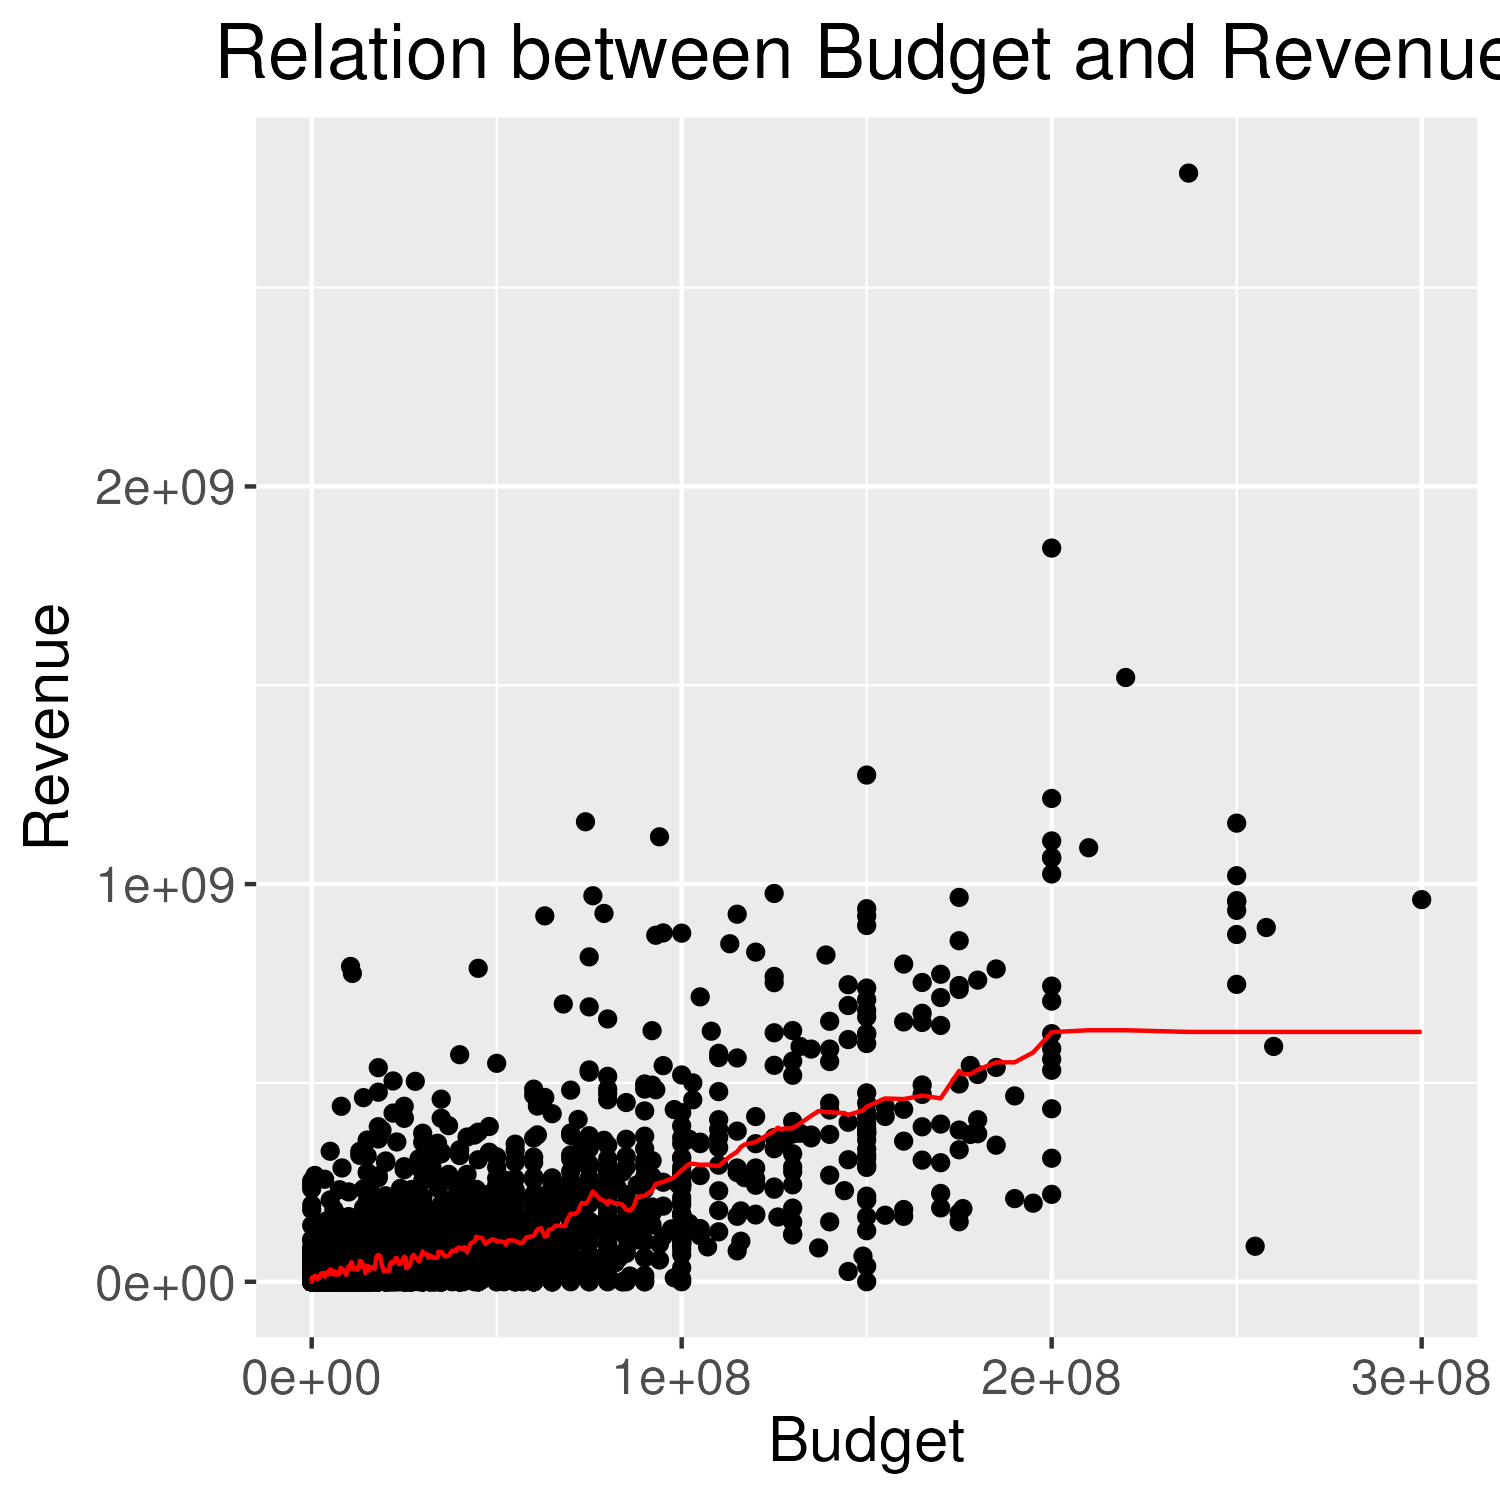
\includegraphics{data/revenue_Budget_plot.jpeg} \#\# Discussion: \#\#\#
Expected outcome

This project centers around studying the profitability of a movie before
it is released, predicting revenues based on budget using Knn
regression. By analyzing the data set, which consists of 5000 movies
from TMDB, a correlation between budget and revenue can be established.
According to the market feedback, a larger production (budget) will
usually indicate higher qualities of production, indicating a higher
revenue. However, as budget exceeds a certain limit, it will reach its
total capacity for revenue feedback due to the limited resources of the
market. Thus, we hypothesize that a revenue and budget will have a
positive correlation, but our model will streamline at a maximum
capacity of revenue since that is the limitation of KNN nearest neighbor
regression(which lose accuracy beyond the range of the training data).

\hypertarget{summary-of-results}{%
\subsubsection{Summary of Results}\label{summary-of-results}}

The result discovered through the model and supports our hypothesis. as
we expected, we found the relationship between the profitability of a
movie and the revenues is positive within the budget range of \(0\) to
\(2*10^8\), after that the slope of the budget and the revenue will go
close to 0, which means our prediction of the revenue will stay constant
as the budget increase. This limitation is caused by the use of KNN
nearest-neighbor regression since it can only predict accurately within
our range. The \(RMSE\) from our result is \(1.316789*10^8\), which is
approximate \(1/10\) of our revenue. This is not a significant mistake,
however this model can be improved further.

We find that the revenue of a film is most closely related to the
investment cost of the film. Therefore, if we want to make the film more
profitable, we have to increase the investment cost of the film to some
extent. KNN regression is very advantageous because it has strong
elasticity to noise and effective data training in the case of training
large amounts of data. We also have a close range of budget with very
few outliers outside of the range so KNN regression works better than
linear regression. By looking at the relationship\_revenue graph, we can
see the correlation between budget and revenue is 0.69, whereas the
others are below 0.6. This is why we use only one predictor in our
project, since others have weak correlation with the target variable. If
we use those weak predictors, the K value will be affected and the
prediction will be less accurate and does not serve our purpose of
prediction. As indicated by the graph ``Relation Between Budget and
Revenue'', it is a perfect fit as it is neither underfitting or
overfitting, thus it will be able to make reasonable prediction to some
extend.

\hypertarget{impact-of-results}{%
\subsubsection{Impact of Results}\label{impact-of-results}}

``Movie revenue depends on multiple factors such as cast, budget, film
critic review, MPAA rating, release year.'' (Apte, 2011). However, due
to the complexity and multi-dimensionality of the multiple factors, an
accurate model is difficult to create with those factors together.
However, by analyzing the relationship between budget and revenue which
have similar range and values, we can visualize trends in production
investment and revenue. Movie production requires large sums of
investment and subsequent effort, so it is crucial to understand how
revenue is linked with budget. By creating this model, we successfully
visualized the correlation and future predictions can be made. Such a
prediction could be very useful for the movie studio which will be
producing the movie so they can decide on expenses like artist
compensations, advertising, promotions, etc. accordingly (Apte, 2011).
Movie theatres will also be able to estimate the revenues they would
generate from screening a particular movie based on given budget.

\hypertarget{future-questions}{%
\subsubsection{Future Questions}\label{future-questions}}

According to our findings, the correlation between revenue and budget is
the strongest. This raises the question - Would a higher budget always
indicate a higher revenue? Besides increasing the budget, we should
think about what other ways we can improve our model to predict the
revenue of the film. The future questions that our research could lead
to is to what extent the increase in budget would affect the revenue of
a movie belonging to a particular genre. Building onto that we can also
do further research to improve the other predictors that can be used for
data analysis. The research can also qualify as a classification problem
if we choose to focus on a particular category of a movie or a
particular production house, and compare which production company
generates greater revenue (Mueller, 2021). Box office trends largely
reflect audience satisfaction with a film. So this raises the question
of whether it's more important to increase the budget, or to focus on
the content and quality of the movie.

\hypertarget{citation}{%
\subsection{Citation}\label{citation}}

(TMDb), T. M. D. (2017, September 28). TMDB 5000 movie dataset. Kaggle.
Retrieved April 7, 2022, from
\url{https://www.kaggle.com/datasets/tmdb/tmdb-movie-metadata}

Mueller, A. (2021, December 1). Why movies cost so much to make.
Investopedia. Retrieved April 7, 2022, from
\url{https://www.investopedia.com/financial-edge/0611/why-movies-cost-so-much-tomake.aspx\#}:\textasciitilde:text=Movie\%20budgets\%20can\%20average\%20around,and\%20special\%20effects\%2C\%20and\%20marketing

Nikhil, A. (2021, December 16). Predicting movie revenue -
cs229.stanford.edu. Predicting Movie Revenue. Retrieved April 8, 2022,
from
\url{https://cs229.stanford.edu/proj2011/ApteForssellSidhwa-PredictingMovieRevenue.pdf}

Mondal, R., Zhang, M., Lu, C., \& Leng, J. (2022). Predicting the
revenue of the movies based on budget. Retrieved 2023, from
\url{https://github.com/rehan13/DSCI-100-Project-Group25.git}

\end{document}
